\documentclass[tikz]{standalone}

%%% Packages
\usepackage{tikz}
\usetikzlibrary{arrows, backgrounds, fit, positioning, shapes, snakes}


%%% Variables
\newcommand{\minwidth}{3cm}
\newcommand{\minheight}{1cm}


%%% tikzstyle
\tikzstyle{terminal} = [% the beginning or end of a program
  ellipse,
  minimum width=\minwidth,
  minimum height=\minheight,
  text centered,
  draw=black,
  fill=red!20
]
\tikzstyle{io} = [% input or output of aata and information
  trapezium,
  trapezium left angle=70,
  trapezium right angle=110,
  minimum width=\minwidth,
  minimum height=\minheight,
  text centered,
  draw=black,
  fill=blue!20
]
\tikzstyle{process} = [% processes: calculations or data manipulations
  rectangle,
  minimum width=\minwidth,
  minimum height=\minheight,
  text centered,
  draw=black,
  fill=brown!20
]
\tikzstyle{decision} = [% decision: comparison, question or decision
  diamond,
  minimum width=\minwidth,
  minimum height=\minheight,
  text centered,
  draw=black,
  fill=green!20
]
\tikzstyle{junction} = [% junction: confluence of flow lines
  circle,
  minimum width=1cm,
  minimum height=1cm,
  text centered,
  draw=black,
  fill=yellow!20
]
\tikzstyle{loop} = [% loop
  chamfered rectangle,
  chamfered rectangle xsep=1cm,
  minimum width=\minwidth,
  minimum height=\minheight,
  draw=black,
  fill=purple!20
  ]
\tikzstyle{group} = [% group format
  fill=gray!20,
  inner sep=15pt
]
\tikzstyle{arrow} = [% arrow format
  ->,
  >=triangle 45,
  thick
]
\tikzstyle{legend} = [% legend format
  minimum width=0.7cm,
  minimum height=0.1cm
]


%%%%%%%%%%%%%%%%%%%%%%%%%%%%%%%%%%%%%%%%%%%%%%%%%%%%%%%%%%%%%%%%%%%%%%%%%%%%%%%
\begin{document}

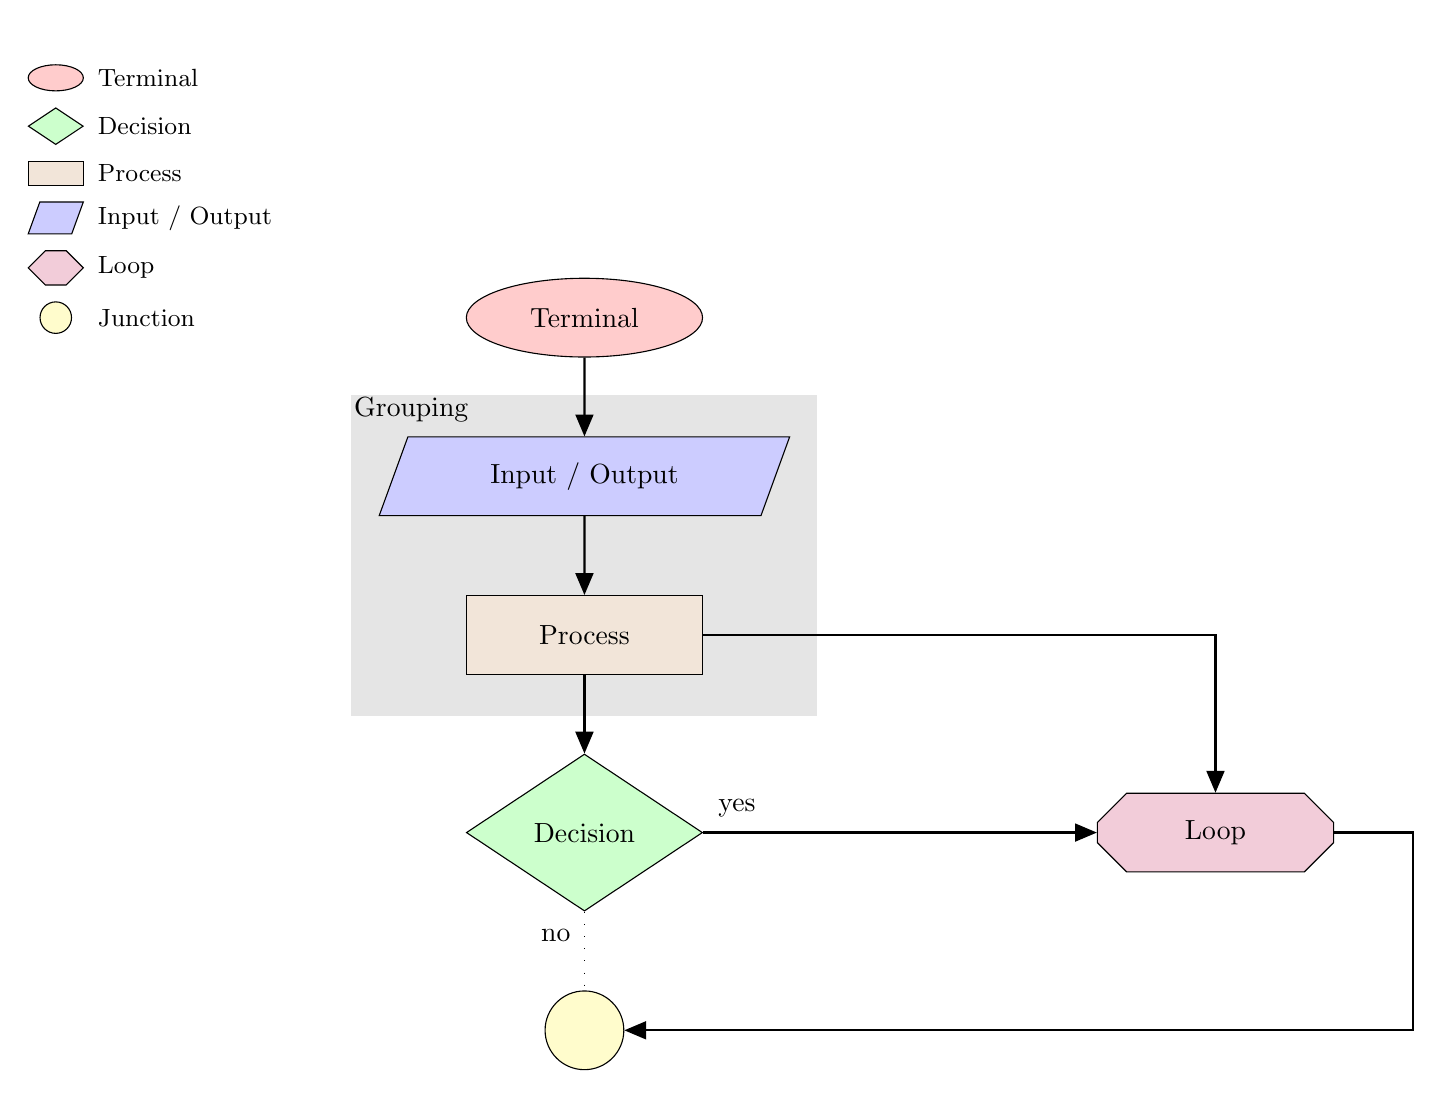
\begin{tikzpicture}[node distance=1cm]

%%% Nodes
\node[terminal] (terminal) {Terminal};
\node[io] (io) [below=of terminal] {Input / Output};
\node[process] (process) [below=of io] {Process};

\node[decision] (decision) [below=of process] {Decision};
\node[text width=1cm] (yes) [above right=1mm of decision.east] {yes};
\node[text width=1.1cm] (no) [below=1mm of decision.south] {no};

\node[junction] (junction) [below=of decision] {};
\node[loop] (loop) [right=5cm of decision] {Loop};


%%% Groupings
\begin{scope}[on background layer]
  \node[group, fit=(io) (process)] (group1) {};
  \node[anchor=north west, inner sep=1pt] at (group1.north west) {Grouping};
\end{scope}


%%% Arrows
\draw[arrow] (terminal) -- (io);
\draw[arrow] (io) -- (process);
\draw[arrow] (process) -- (decision.north);
\draw[loosely dotted] (decision.south) -- (junction);
\draw[arrow] (decision.east) -- (loop.west);
\draw[arrow] (loop.east) -- ++(1, 0) |- (junction.east);
\draw[arrow] (process.east) -| (loop.north);


%%% Legend
\node[junction, legend, minimum width=0.4cm] (LegendJunction) [left=5cm of terminal] {};
\node[anchor=west, inner sep=15pt] at (LegendJunction) {\small Junction};

\node[loop, legend] (LegendLoop) [above=0.2cm of LegendJunction] {};
\node[anchor=west, inner sep=15pt] at (LegendLoop) {\small Loop};

\node[io, legend] (LegendInputOutput) [above=0.2cm of LegendLoop] {};
\node[anchor=west, inner sep=15pt] at (LegendInputOutput) {\small Input / Output};

\node[process, legend, minimum height=0.3cm] (LegendProcess) [above=0.2cm of LegendInputOutput] {};
\node[anchor=west, inner sep=15pt] at (LegendProcess) {\small Process};

\node[decision, legend] (LegendDecision) [above=0.2cm of LegendProcess] {};
\node[anchor=west, inner sep=15pt] at (LegendDecision) {\small Decision};

\node[terminal, legend] (LegendStartStop) [above=0.2cm of LegendDecision] {};
\node[anchor=west, inner sep=15pt] at (LegendStartStop) {\small Terminal};

\end{tikzpicture}

%%%%%%%%%%%%%%%%%%%%%%%%%%%%%%%%%%%%%%%%%%%%%%%%%%%%%%%%%%%%%%%%%%%%%%%%%%%%%%%
\end{document}
